\section{Durchführung}
\label{sec:Durchführung}
\subsection{Entladevorgang des RC-Kreises und Bestimmung der Zeitkonstanten}
\label{sec:Lade}
\begin{figure}
    \centering
    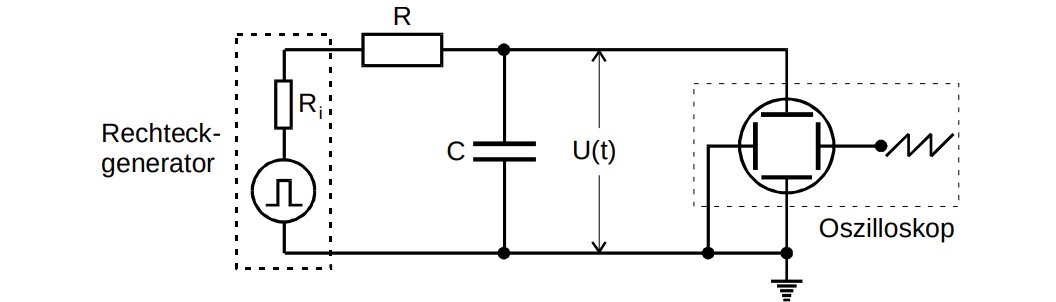
\includegraphics[width=10cm]{content/Schaltbild.png}
    \caption{Messung des Entladevorgangs eines RC-Gliedes \cite{sample}}
\end{figure}
\noindent Um den Entladevorgang des RC-Gliedes mit Wert 1 zu untersuchen,
wird die Spannung am Kondensator mit Hilfe eines
Oszilloskopes beobachtet. An das RC-Glied wird ein 
Generator angeschlossen, welcher eine Rechteckspannung
mit einer Amplitude von $U_0=4,8\,\symup{V}$ erzeugt.
Sobald der Kondensator voll aufgeladen ist und die Spannung
auf null springt, beginnt die Entladung des Kondensators.
Der Vorgang endet, wenn die Spannung wieder $U=U_0=4,8\,\symup{V}$
beträgt. Der Entladevorgang kann also nicht vollständig
aufgezeichnet werden, das Oszilloskop zeigt jedoch
einen entsprechenden Ausschnitt (REFERENZ BILD) mit dem
sich die Zeitkonstante RC bestimmen lässt.


\subsection{Frequenzabhängigkeit der Phasenverschiebung und der Amplitude beim Kondensator}
\label{sec:freq}
\begin{figure}
    \centering
    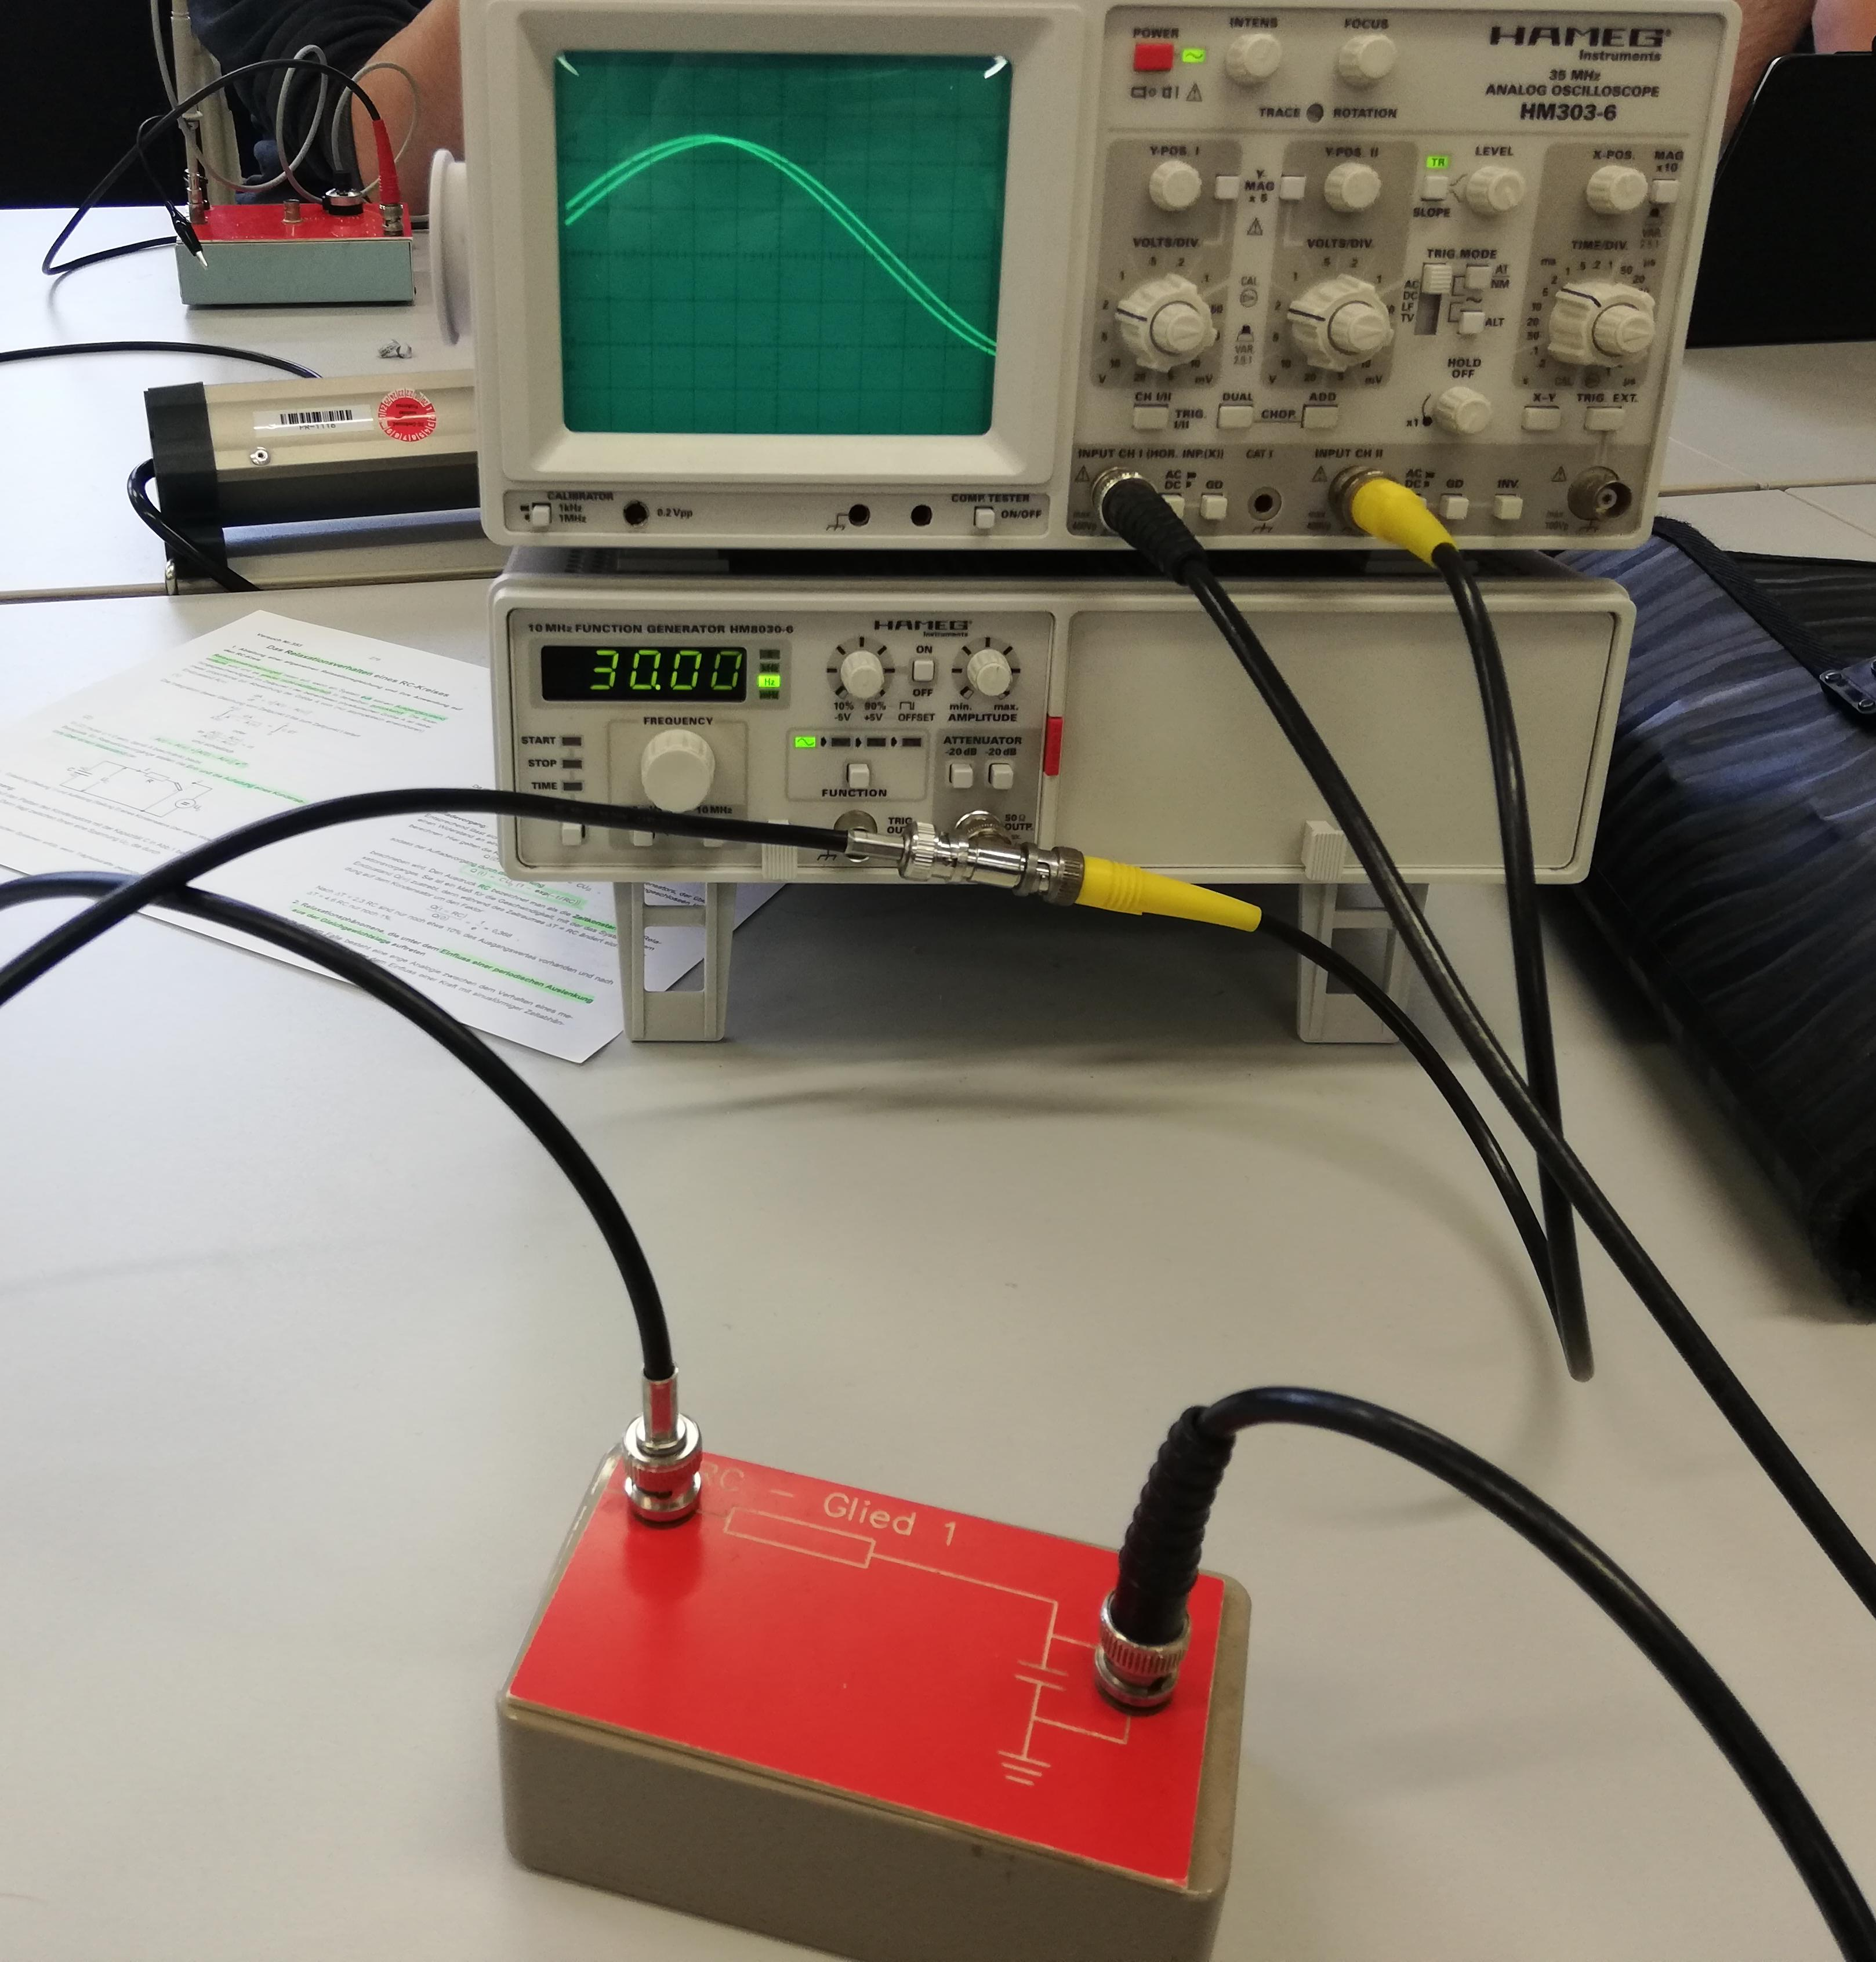
\includegraphics[width=10cm]{content/Aufbau.jpg}
    \caption{Aufbau zur Messung der Frequenzabhängigkeit der Phasenverschiebung und der Amplitude beim Kondensator}
\end{figure}
\noindent Der Aufbau entspricht dem von \ref{sec:Lade} wobei hier
zusätzlich die Spannung $U$ des Generators auf dem
zweiten Kanal des Oszillographen angezeigt wird und
somit mit der Spannung $U_C$ des Kondensators verglichen
werden kann. Außerdem liegt nun keine Rechteckspannung,
sondern eine Sinusspannung mit $U_0=5\,\symup{V} $ vor.
Die Phasenverschiebung $\phi$ zwischen $U$ und $U_C$
und die Amplitude von $U_C$ werden nun gleichzeitig
untersucht. Dafür wird die Frequenz $\omega$ der
Generatorspannung $U$ von 10\,Hz bis 10\,000\,Hz
hochgeregelt und 21 Messwerte ins Messheft aufgenommen.

\subsection{Integrierfunktion des RC-Kreises}
Es wird der gleiche Aufbau wie bei \label{sec:freq} verwendet.
Nach der Bedingung $\omega \gg 1$/$RC$ wird
eine Frequenz von $\omega=45\,\symup{kHz}$ gewählt.
Anschließend soll die zu integrierende und integrierte
Spannung auf dem Zweikanaloszilloskop bei einer
Rechteck-, Sinus- und Dreieckspannung dargestellt werden.
Die Amplitude der Generatorspannung $U$ ist hierbei
5\,V.

